\section{Hiểu dữ liệu (Data Understanding)}
\label{sec:b}

Phần A của bước này (``mù'') chỉ đọc D3 và data dictionary: tổng quan, thống kê mô tả, phân phối, giá trị thiếu, tương quan, ngoại lai bằng sáu phương pháp và phân tích khoảng cách/mật độ. Phần B mới đọc D0--D2 và nhật ký chèn lỗi,
để đo tác động từng thao tác và kiểm chứng các phát hiện mù.

\subsection{Tổng quan và phân phối}
D3 có 260 dòng $\times$ 14 thuộc tính (cùng \var{customer_id} duy nhất, không dòng trùng). Khoảng giá trị thực tế \emph{vượt miền khai báo} ở nhiều cột (tuổi tới 150, thời lượng phiên 1440 phút, số phiên 999).
Mười cột số đều lệch phải ở mức khác nhau (Bảng~\ref{tab:desc}); 80 khách (30,8\%) chỉ có đúng 1 đơn và 11 khách chạm trần recency 365 ngày.

\begin{table}[htbp]
\centering\small
\caption{Thống kê mô tả của D3 (chưa xử lý). Tỉ số $s/s_{\mathrm{bền}}$ là độ lệch chuẩn chia độ lệch chuẩn bền (IQR/1,349): lớn nghĩa là vài giá trị cực trị làm phồng độ lệch chuẩn.}
\label{tab:desc}
\begin{tabular}{lrrrrrr}
\toprule
Thuộc tính & Trung vị & Trung bình & Skew & $s/s_{\mathrm{bền}}$ & Lớn nhất\\
\midrule
\var{age} & 32 & 33,6 & 3,33 & 1,15 & 150\\
\var{n_orders_12m} & 5 & 15,5 & 3,33 & 1,93 & 178\\
\var{avg_order_value} & 43,8 & 86,9 & 9,19 & 10,62 & 3\,093\\
\var{total_spend_12m} & 211,7 & 1\,455 & 8,52 & 9,33 & 62\,272\\
\var{recency_days} & 42 & 81,3 & 1,69 & 1,53 & 365\\
\var{discount_usage_rate} & 0,21 & 0,39 & 0,83 & 0,65 & 1,80\\
\var{sessions_per_month} & 10,05 & 14,9 & 15,70 & 7,67 & 999\\
\var{avg_session_minutes} & 8,5 & 18,9 & 14,84 & 11,14 & 1\,440\\
\var{pages_per_session} & 7,2 & 10,5 & 1,64 & 1,40 & 46,7\\
\var{cart_abandon_rate} & 0,42 & 0,52 & 0,74 & 0,83 & 1,35\\
\bottomrule
\end{tabular}
\end{table}

\subsection{Giá trị thiếu}
Ba cột có giá trị thiếu: \var{age} 21 ô (8,1\%), \var{avg_session_minutes} 31 ô (11,9\%), \var{preferred_category} 13 ô (5,0\%). Tổng cộng 61/260 dòng (23,5\%) có ít nhất một ô thiếu, nên xóa dòng sẽ mất gần một phần tư dữ liệu.
Tỉ lệ thiếu của \var{avg_session_minutes} khác nhau theo thiết bị (desktop 21,8\%, tablet 12,2\%, mobile 6,4\%); kiểm định hoán vị cho $p = 0{,}0037$ \emph{nhưng sau hiệu chỉnh Bonferroni cho 39 phép thử là $p = 0{,}144$}, nghĩa là
dấu hiệu MAR có nhưng chưa vượt được đa phép thử. Với \var{preferred_category}, kiểm định $\chi^2$ cho $p = 0{,}0006$ nhưng số kỳ vọng nhỏ nhất chỉ 2,05 ($<5$) nên xấp xỉ không đáng tin; kiểm định hoán vị cho $p = 0{,}0015$, Bonferroni $0{,}0585$, tức chưa đủ bằng chứng.

\begin{figure}[htbp]
\centering
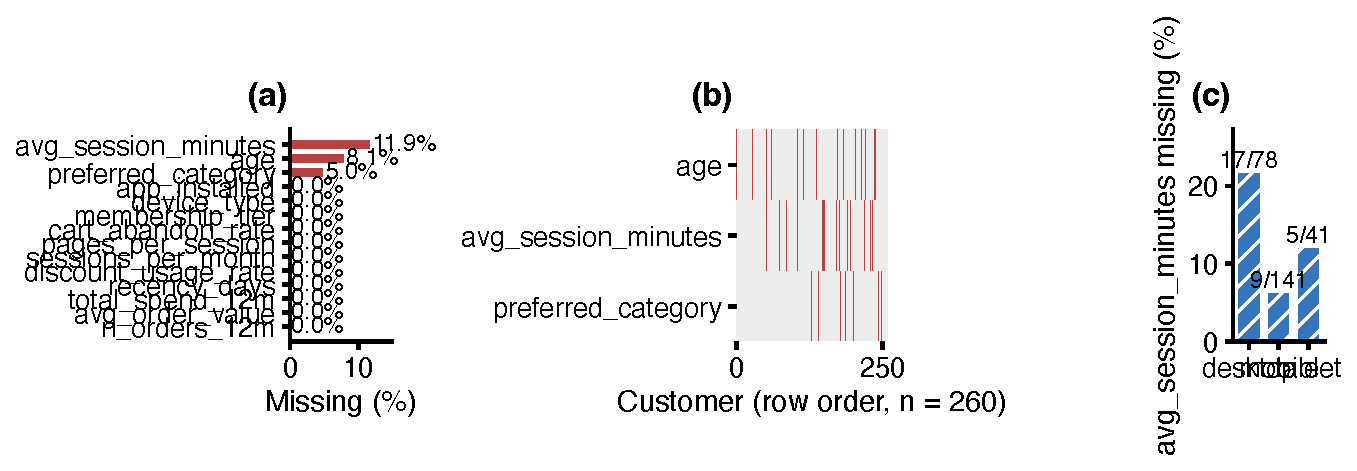
\includegraphics[width=\linewidth]{fig02_missing_values.pdf}
\caption{Giá trị thiếu trong D3. (a) Tỉ lệ thiếu theo cột. (b) Vị trí ô thiếu theo từng khách: không có mẫu thiếu theo khối. (c) Tỉ lệ thiếu của \var{avg_session_minutes} theo thiết bị.}
\label{fig:b_missing}
\end{figure}

\subsection{Quan hệ giữa các thuộc tính}
Tương quan hạng Spearman cho thấy các cặp mạnh: \var{n_orders_12m} $\sim$ \var{total_spend_12m} ($0{,}92$), \var{avg_session_minutes} $\sim$ \var{pages_per_session} ($0{,}85$),
\var{n_orders_12m} $\sim$ \var{recency_days} ($-0{,}75$), \var{sessions_per_month} $\sim$ \var{pages_per_session} ($0{,}74$). Hệ số VIF trên hạng của \var{total_spend_12m} và \var{n_orders_12m} đều xấp xỉ 23; ma trận tương quan cần 3 thành phần để giữ 80\% và 5 thành phần để giữ 90\% phương sai (trên 10 biến số),
nghĩa là số chiều hiệu dụng chỉ bằng khoảng một nửa số cột.
Điểm đáng chú ý nhất là \textbf{Pearson thô và Spearman lệch nhau rất nhiều} do các ô hỏng: tương quan giữa thời lượng phiên và số trang là $0{,}049$ theo Pearson nhưng $0{,}848$ theo Spearman (Hình~\ref{fig:b_corr}).
Ở dữ liệu sạch, cùng cặp này có Pearson $0{,}906$: ô hỏng đã phá hủy quan hệ tuyến tính.

\begin{figure}[htbp]
\centering
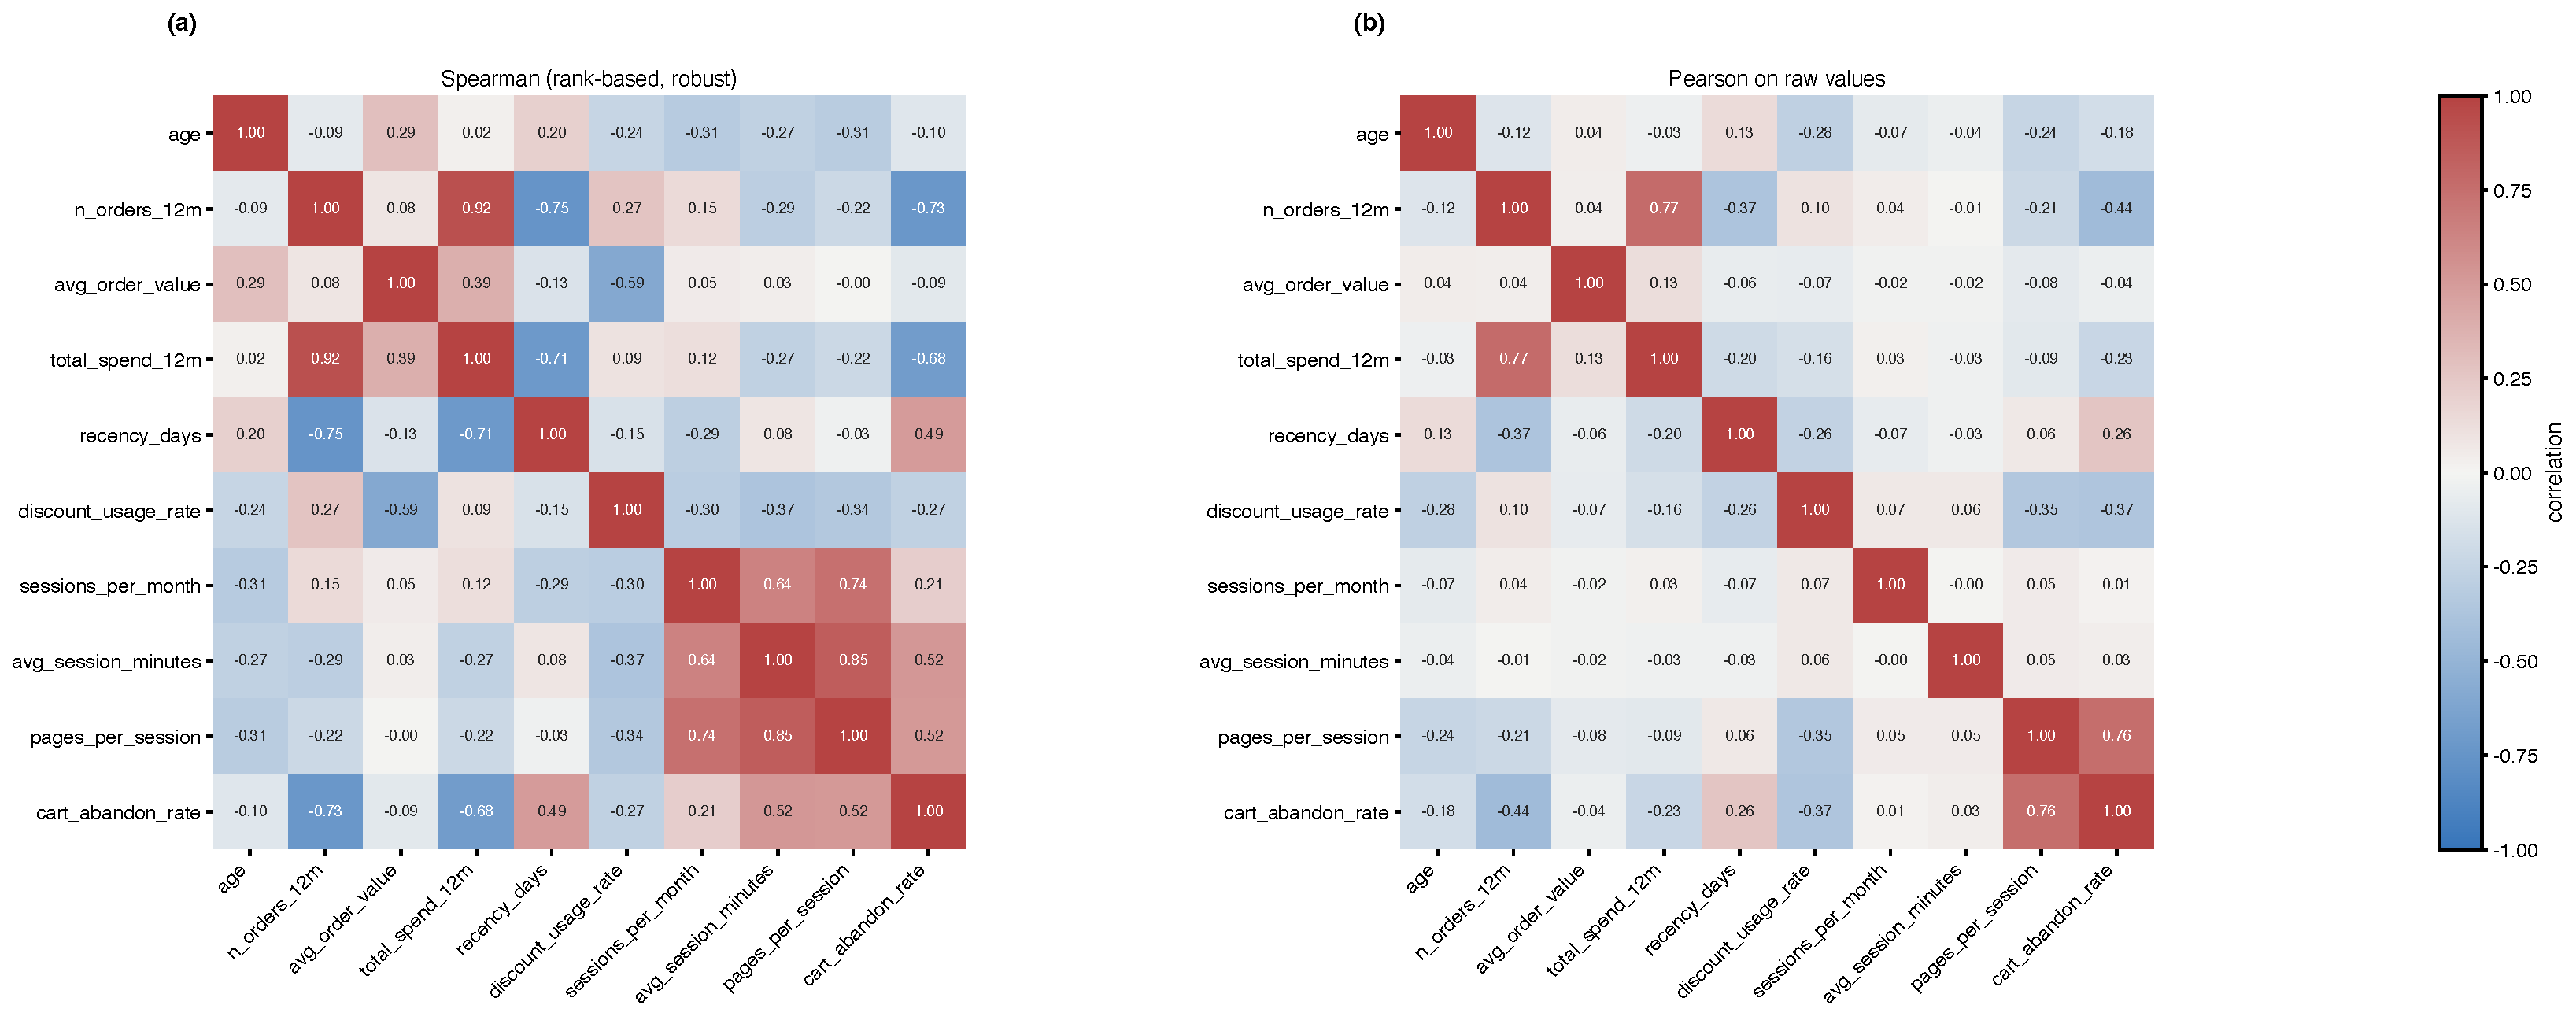
\includegraphics[width=\linewidth]{fig08_correlation_numeric.pdf}
\caption{Ma trận tương quan 10 biến số của D3: (a) Spearman (dựa hạng, bền); (b) Pearson trên giá trị thô. Các cặp có liên quan tới \var{sessions_per_month} và \var{avg_session_minutes} gần như mất tương quan ở (b).}
\label{fig:b_corr}
\end{figure}

\subsection{Giá trị bất thường}
Sáu phương pháp cho kết quả rất khác nhau (Bảng~\ref{tab:outlier}). Luật miền nghiệp vụ cộng với kiểm tra đẳng thức xấp xỉ $\mathrm{total}\approx\mathrm{n\_orders}\times\mathrm{AOV}$ gắn cờ đúng 7 dòng lỗi,
trong khi Tukey $1{,}5$ IQR gắn cờ 94 dòng (36,2\%) chỉ vì phân phối lệch phải. Sau khi đối chiếu với nhật ký (Phần B), độ chính xác (precision) của Tukey $1{,}5$ chỉ là $0{,}14$, và phương pháp thống kê chung gắn cờ cả 8 khách cực trị \emph{hợp lệ}
cùng hàng chục dòng bình thường. Do đó không thể dùng một ngưỡng thống kê để xóa ngoại lai.

\begin{table}[htbp]
\centering\small
\caption{Phát hiện ngoại lai ở Phần A (mù) và kiểm chứng ở Phần B với 15 khách thực sự bị chèn (8 hợp lệ, 7 lỗi).}
\label{tab:outlier}
\begin{tabular}{lrrrrr}
\toprule
Phương pháp & Số dòng gắn cờ & Bắt được & Precision & Recall lỗi (7) & Recall hợp lệ (8)\\
\midrule
Luật miền + đẳng thức & 7 & 7 & 1,00 & 7/7 & 0/8\\
Tukey $1{,}5$ IQR & 94 & 13 & 0,14 & 5/7 & 8/8\\
Tukey $3$ IQR & 38 & 12 & 0,32 & 4/7 & 8/8\\
Robust $z>3{,}5$ (trên log) & 33 & 10 & 0,30 & 6/7 & 4/8\\
LOF ($k=20$) & 10 & 9 & 0,90 & 6/7 & 3/8\\
\bottomrule
\end{tabular}
\end{table}

\subsection{Các vấn đề dữ liệu chính và tác động đo được lên khoảng cách, mật độ và cấu trúc cụm}
Vì phân cụm dựa vào khoảng cách, phần quan trọng nhất là xem các vấn đề dữ liệu làm thay đổi hình học thế nào (Hình~\ref{fig:b_dist}, Bảng~\ref{tab:stages}):
\begin{itemize}
\item \textbf{Thang đo và ô hỏng quyết định khoảng cách.} Khi không chuẩn hóa, \var{total_spend_12m} chiếm 99,59\% tổng phương sai. Sau z-score thô, 7 dòng lỗi (2,7\% số dòng) vẫn chiếm 31,4\% tổng bình phương khoảng cách của mọi cặp;
một ô \var{sessions_per_month}=999 kéo độ lệch chuẩn cột này lên 61,8 so với 8,1 theo thang bền, nén 259 dòng còn lại về gần hằng số ở cột đó.
\item \textbf{Lân cận cục bộ rất nhạy.} Chỉ riêng nhiễu đã làm mất 21--33\% lân cận 5-NN dù phân phối biên gần như không đổi (thống kê KS $0{,}03$--$0{,}05$); thêm ngoại lai còn $0{,}53$--$0{,}62$ lân cận được giữ lại.
\item \textbf{Thống kê Hopkins bị phồng khi có ngoại lai} (từ $0{,}83$ lên $0{,}94$ với z-score thô) do khung dữ liệu bị kéo giãn, nên không đáng tin để kết luận ``dữ liệu có cụm'' trên D3.
\item \textbf{Phân phối lệch phải nặng với biên cứng.} Trung bình gấp $6{,}9$ lần trung vị với \var{total_spend_12m} và $3{,}1$ lần với \var{n_orders_12m}; 7/10 cột có độ lệch $>1$ sau khi loại các ô vi phạm miền; 80 khách (30,8\%) dồn ở đúng 1 đơn.
Hệ quả đo được: ngay cả sau z-score thô, 5 dòng lớn nhất vẫn nắm $21{,}9\%$ tổng bình phương độ lệch và $17$ ô vượt $4$ độ lệch chuẩn (Bảng~\ref{tab:scaler}); sau log1p con số này là $6{,}6\%$ và $2$ ô.
\item \textbf{Thông tin trùng lặp.} Số đơn và tổng chi có Spearman $0{,}92$ (VIF $\approx 23$); trên thang log, tổng chi được giải thích gần hết bởi số đơn và giá trị đơn ($R^2 = 0{,}987$); ma trận tương quan chỉ cần 3--5 thành phần cho 80--90\% phương sai.
Nghĩa là các trục này bị đếm nhiều lần trong khoảng cách.
\item \textbf{Giá trị thiếu ở 23,5\% số dòng.} Xóa dòng làm mất 61 khách; tỉ lệ thiếu của thời lượng phiên chênh theo thiết bị ($6{,}4\%$ đến $21{,}8\%$) nên xóa dòng còn làm lệch cơ cấu thiết bị.
\item \textbf{Độ tách phân khúc giảm}: Silhouette theo nhãn ẩn (chỉ chẩn đoán) giảm từ $0{,}327$ xuống $0{,}288$ trên biểu diễn log1p + median/IQR.
\end{itemize}

\begin{figure}[htbp]
\centering
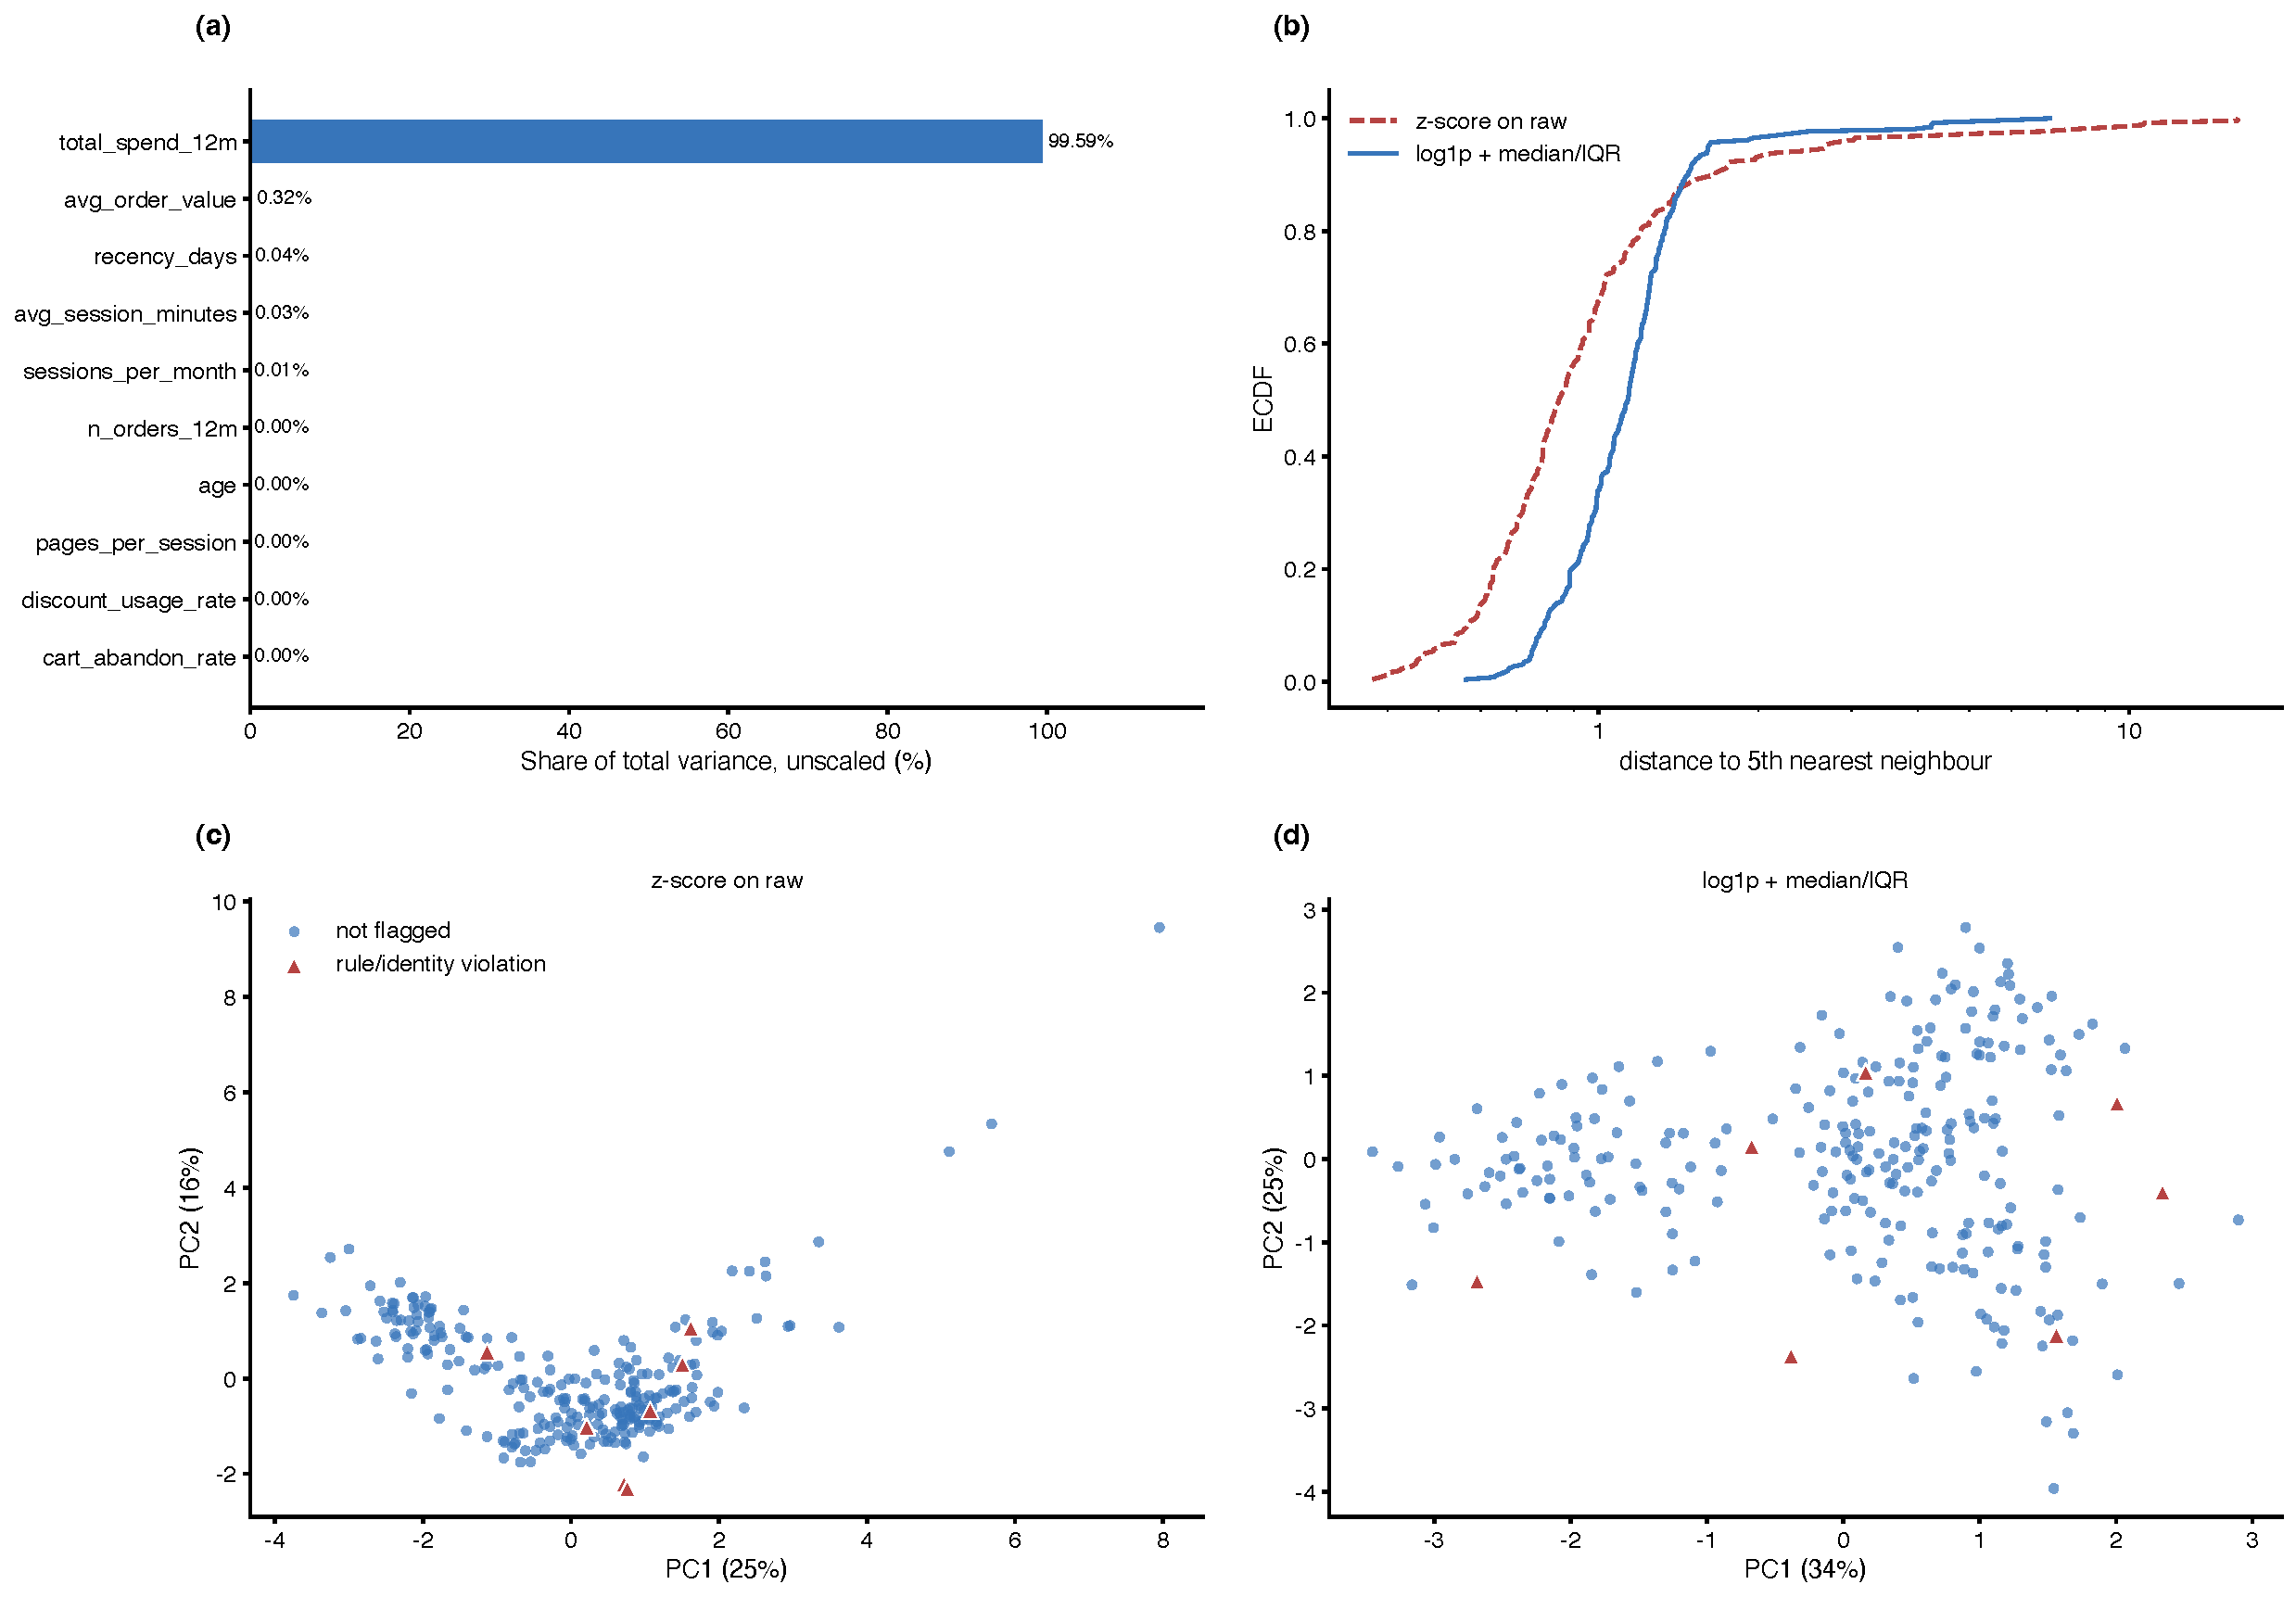
\includegraphics[width=0.92\linewidth]{fig12_distance_and_density.pdf}
\caption{Tác động lên khoảng cách và mật độ (D3). (a) Phần phương sai thô của từng thuộc tính: một cột chiếm 99,6\%. (b) ECDF khoảng cách tới láng giềng thứ 5: đuôi rất dài với z-score thô.
(c, d) Chiếu PCA 2 chiều: các dòng vi phạm luật miền/đẳng thức (tam giác) bị đẩy ra xa ở z-score thô, ít hơn ở log1p + median/IQR.}
\label{fig:b_dist}
\end{figure}

\begin{table}[htbp]
\centering\small
\caption{Cấu trúc qua bốn giai đoạn dữ liệu (so với D0). Mỗi ô: z-score thô / log1p + median/IQR.}
\label{tab:stages}
\begin{tabular}{lcccc}
\toprule
Giai đoạn & 5-NN giữ lại & Tương quan hạng khoảng cách & Hopkins & Silhouette (nhãn ẩn)\\
\midrule
D0 sạch & 1,00 / 1,00 & 1,00 / 1,00 & 0,833 / 0,724 & 0,298 / 0,327\\
D1 + nhiễu & 0,79 / 0,67 & 0,99 / 0,98 & 0,837 / 0,718 & 0,294 / 0,317\\
D2 + ngoại lai & 0,55 / 0,62 & 0,78 / 0,87 & 0,939 / 0,835 & 0,281 / 0,297\\
D3 + thiếu & 0,53 / 0,57 & 0,77 / 0,86 & 0,940 / 0,835 & 0,281 / 0,288\\
\bottomrule
\end{tabular}
\end{table}
\FloatBarrier
